\documentclass{article}
\usepackage{blindtext}
\usepackage[utf8]{inputenc}
\usepackage[english]{babel}

\usepackage{comment}

\usepackage{graphicx}
\graphicspath{ {fig/} }
\usepackage{placeins}

\usepackage{cite}

\begin{document}
\title{MESF6910J, Term 2, 2017-2018\\Final Project Report}
\author{Kaiwen Chen\thanks{Kaiwen Chen
\newline kchenau@connect.ust.hk
\newline
\newline Department of Mechanical and Aerospace Engineering
\newline Master of Science in Aeronautical Engineering
\newline Hong Kong University of Science and Technology
\newline Clear Water Bay, Kowloon, Hong Kong}}
\date{\today}

\maketitle

\section{Case Desciption}
The MBB structure is considered with one Newtown load at the middle point in its top surface. The material has a modulus of elasticity of 100 MPa and the Poisson’s ratio of 0.3. The 3D SIMP topology optimization method is conducted for the minimization of the strain energy function c, defined as:\\
$$c(\tilde{x})=F^TU(\tilde{x}) $$

where x is the physical densities, F is the nodal force vector and $U(\tilde{x})$ is the vector of nodal displacements. The nodal force vector F is independent of the design variables and the nodal displacement vector $U(\tilde{x})$ is the solution of $K(\tilde{x})U(\tilde{x})=F$

The detail problem can be described as follows: MBB beam is supported at the four corns in its bottom surface. The support is a three-dimensional planar joint. The unit force (1 Newtown) is exerted at the middle point in its top surface and heading to downward directly. The coordinate origin is placed at the left-bottom-back corner. The Cartesian coordinate system follows the right-hand rule with its x axis follow the longitude direction. The design domain has the scale $6L\times L\times L$ with L equals to 1.0cm i.e. the domain is a cuboid with the size of $60mm\times10mm\times10mm$. The mesh is $120\times20\times20$. The volume fraction is set as 0.2 and penalization factor is set as 3.


\begin{figure}[!htb]
\centering
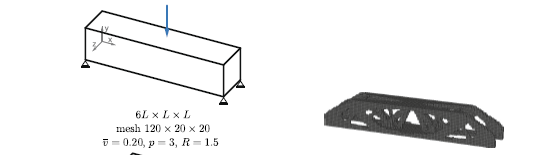
\includegraphics[width=0.5\textwidth]{CaseDescription}
\caption{Case Descrption}
\end{figure}
\FloatBarrier



\section{Methodology}

A 3D SIMP topology optimization code written in MATLAB called Top3d is given at \emph{https://top3dapp.com}. The method is described  in the paper
\begin{quote} 
\textit{K. Liu and A. Tovar, "An efficient 3D topology optimization code written in Matlab", Struct Multidisc Optim, 50(6): 1175-1196, 2014, doi:10.1007/s00158-014-1107-x}~\cite{liu2014efficient}.
\end{quote}
It is written intending for engineering education. The state variables and boundary condition are defined in the Matlab code. They are modified to this case by the author. 



\section{Alternative Filters Study-Searching for the most black-and-white solution}
To avoid numerical instabilities like checkerboard, different kinds of filters have been introduced. Different filtering techniques can result in different discreteness of final solutions and eventually cause different topology. In this case study, three different kinds of filters are implemented individually or combinedly. They are 
\begin{enumerate} 
\item{density filter} 
\item{sensitivity filter} 
\item{gray scale filter} 
\end{enumerate} 

Density filter and sensitivity filter have been studied in the Mid-term project report. Here we briefly discuss the gray scale filter and then compare the results of these filtering techniques.

Gray scale filter is a simple non-linear gray-scale filter proposed by Groenwold and Etman \cite{groenwold2009} to further achieve black-and-white topologies. The implementation of gray scale filter is by changing the OC update scheme as the following:

$$ x_i^{new}=\left\{
\begin{array}{rlc}
max(0,x_i-m) & if & {x_iB_i^\eta\leq max(0,x_i-m)}\\
min(1,x_i+m) & if & {x_iB_i^\eta\geq min(1,x_i-m)}\\
(x_iB_i^\eta)^q & &{otherwise}\\
\end{array} \right. $$


The standard OC updating method is a special case with $q=1$. For the SIMP-based topology optimization the value of q is $q = 2$. The factor q should be increased gradually from the small value 1 to 2. In the program, the first fifteen loops use q equals to 1. After the fifteenth loop, q is increased by 1 percent in each loop until it equals to 2. 
\subsection{Density filter only}

\begin{figure}[!htbp]
\centering
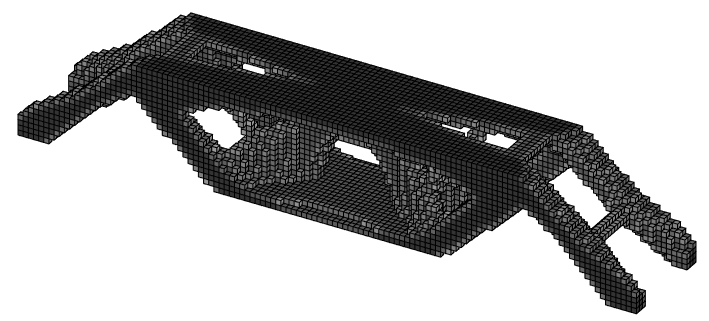
\includegraphics[width=1\textwidth]{Densityfilteronly}
\caption{Result of density filter only}
\end{figure}
\FloatBarrier

\subsection{Sensitivity filter only}

\begin{figure}[!htbp]
\centering
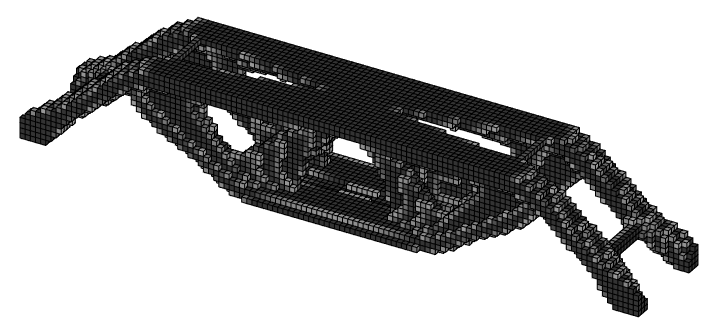
\includegraphics[width=1\textwidth]{Sensitivityfilteronly}
\caption{Result of sensitivity filter only}
\end{figure}
\FloatBarrier

\subsection{Grey scale filter only}

\begin{figure}[!htb]
\centering
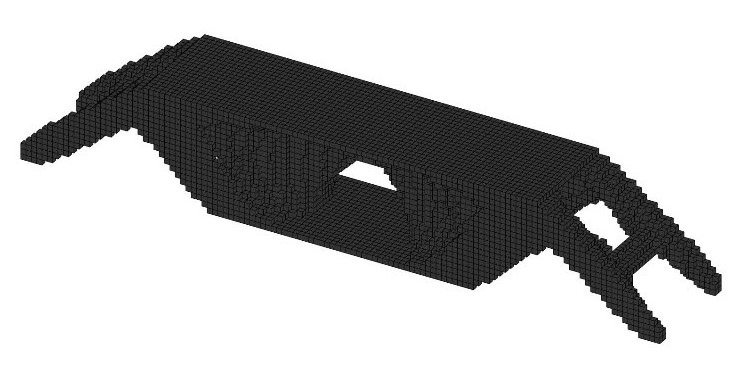
\includegraphics[width=1\textwidth]{Greyscalefilteronly}
\caption{Result of grey scale filter only}
\end{figure}
\FloatBarrier

\subsection{Density filter and grey scale filter}

\begin{figure}[!htb]
\centering
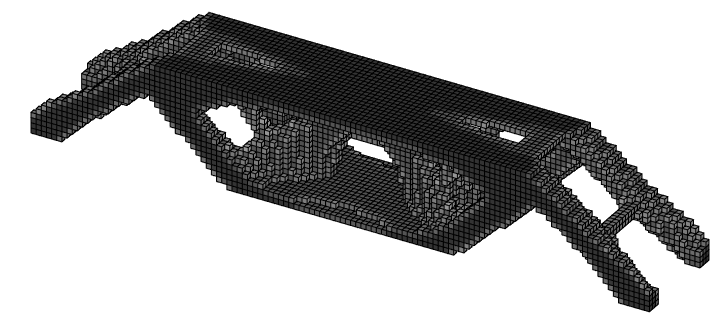
\includegraphics[width=1\textwidth]{Densityfilterandgreyscalefilter}
\caption{Result of density filter and grey scale filter}
\end{figure}
\FloatBarrier

\subsection{Sensitivity filter and grey scale filter}

\begin{figure}[!htb]
\centering
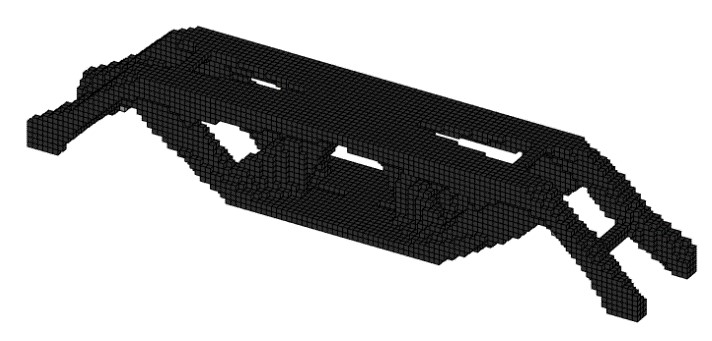
\includegraphics[width=1\textwidth]{Sensitivityfilterandgreyscalefilter}
\caption{Result of sensitivity filter and grey scale filter}
\end{figure}
\FloatBarrier

According to the result figure, the Sensitivity filter and grey scale filter provides the most black-and-white solution.

\section{3D Printing}

The model is the optimization result using the sensitivity filter and grey scale filter, which is the most black-and-white solution from the analysis above. The STL writing program use the unitlength of [0.5 0.5 0.5] since the mesh is $120\times20\times20$ and the design domain is $60mm\times10mm\times10mm$ which means the element unit length should be 0.5mm. The file is written in ‘binary’ for machine-readable. The density cutoff value leaves as 0.5.


There are two facet representations: Cubic representation and ISO representation. Both should be studied independently. Two models have been printed.
\begin{figure}[!htb]
\centering
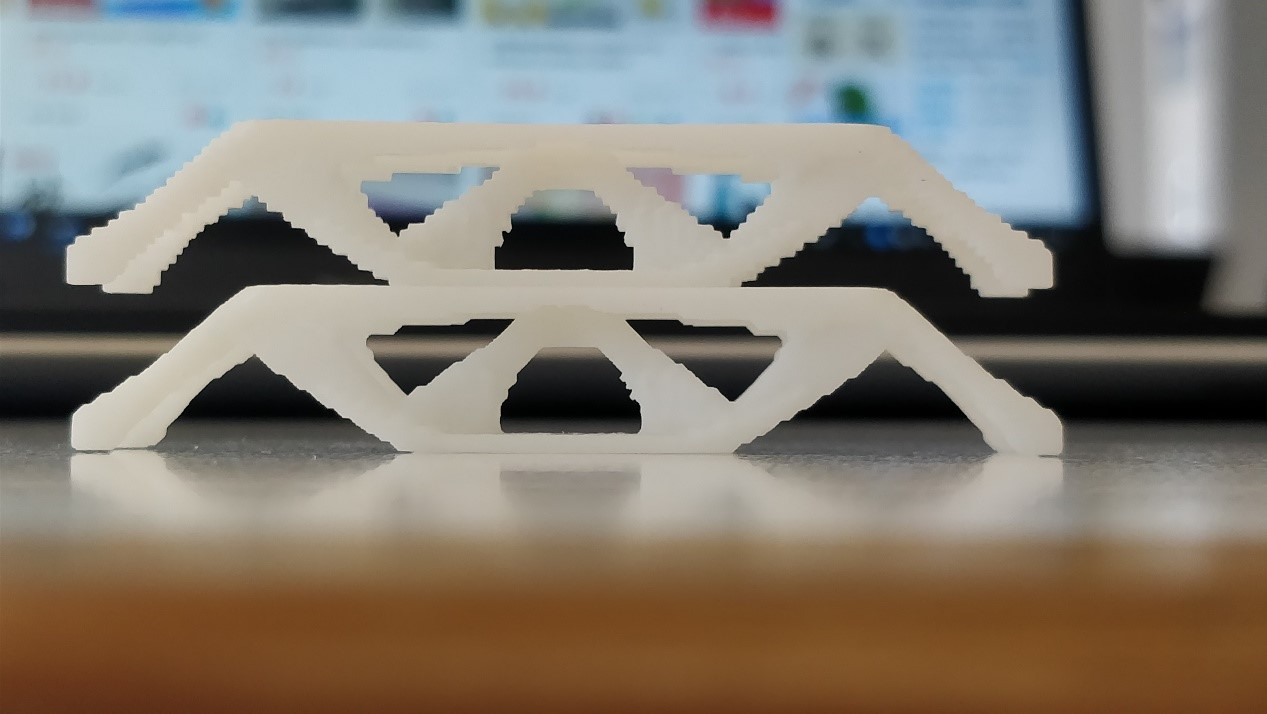
\includegraphics[width=1\textwidth]{CameraPhoto}
\caption{3D-Printed model	Top: Cubic representation	Bottom: ISO representation}
\end{figure}

\begin{figure}[!htb]
\centering
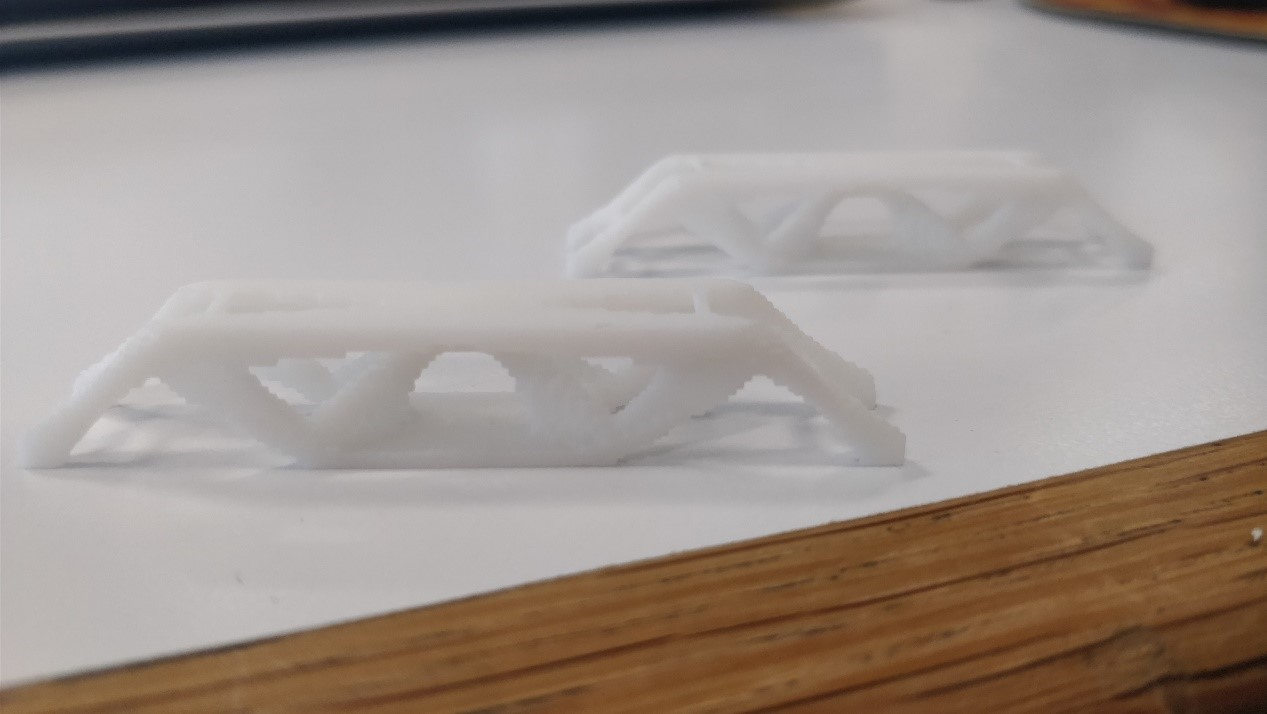
\includegraphics[width=1\textwidth]{3Dmodel}
\caption{3D-Printed model	Left: Cubic representation 	Right: ISO representation}
\end{figure}
\FloatBarrier
As we can see from the pictures, the ISO reprensentation has much smoother surface. The border changes slightly. The border of cubic representation is zigzag. Almost all the angles are 90 degree.
\subsection{Printing method: SLA}

The printer uses stereolithography(SLA) method to print this model.SLA is a form of 3D printing technology. It creates models, prototypes, patterns and production of parts in a layer by layer fashion using photopolymerization. Photopolymerization is a process by which light causes chains of molecules to link, forming polymers. Those polymers then make-up the body of a three-dimensional solid.

\subsection{3D Printer: UnionTech Lite 600 3D Printer\cite{UnionTech}}

Manufacturing accuracy: $\pm0.1 mm$\\
Layer thickness: 0.05 - 0.25 mm\\
Z axis positioning accuracy: $\leq \pm8 \mu m$

\begin{figure}[!htb]
\centering
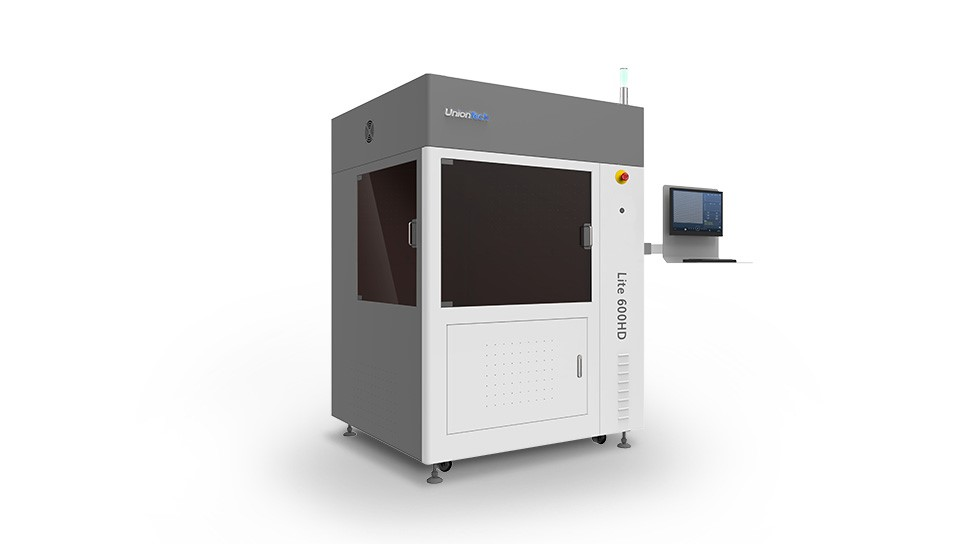
\includegraphics[width=1\textwidth]{3DPrinter}
\caption{UnionTech Lite 600 3D Printer}
\end{figure}
\FloatBarrier
\subsection{Resin material: DSM Somos® 14120}
DSM’s Somos® 14120\cite{Somos14120} is a low-viscosity liquid photopolymer that produces strong, tough and water-resistant parts. Parts created with Somos® 14120 have a white, opaque appearance similar to production plastics.

This ABS-like photopolymer is used in solid imaging processes, like stereolithography, to build three-dimensional parts. Somos® 14120 offers many properties that mimic traditional engineering plastics, including ABS and PBT. This makes the material ideal for many applications in the automotive, medical and consumer electronics markets and include functional prototypes, water-resistant applications, appearance models with minimal finishing, durable concept models, high humidity environment applications and RTV patterns

\medskip
\bibliographystyle{unsrt}
\bibliography{sample}


\end{document}


